\documentclass[journal]{IEEEtran}
\usepackage{amsmath,amsfonts}
\usepackage{algorithmic}
\usepackage{algorithm}
\usepackage{amssymb}
\usepackage{array}
\usepackage[caption=false,font=normalsize,labelfont=sf,textfont=sf]{subfig}
\usepackage{textcomp}
\usepackage{stfloats}
\usepackage{url}
\usepackage{verbatim}
\usepackage{graphicx}
\usepackage{cite}
\usepackage{xcolor}
\hyphenation{op-tical net-works semi-conduc-tor IEEE-Xplore}
\usepackage{hyperref}
\hypersetup{
  colorlinks=true,   % Enable colored links
  linkcolor=blue,    % Set internal links to blue
  citecolor=blue,    % Set citation links to blue
  urlcolor=blue      % Set URL links to blue
}
\usepackage{booktabs} % for \hline
\renewcommand{\algorithmicrequire}{\textbf{Input:}}
\renewcommand{\algorithmicensure}{\textbf{Output:}}
\usepackage{threeparttable}
\usepackage{amsthm}
\newtheorem{definition}{Definition}
\newtheorem{proposition}{Proposition}
\usepackage{listings}
\usepackage{tikz}
\usetikzlibrary{shapes,arrows,positioning,calc,shadows,decorations.pathreplacing,fit}
\usepackage{multirow}

\begin{document}

\title{Thread-Adaptive: Optimized Parallel Architectures of SLH-DSA on GPUs}

\author{Jiahao Xiang and Lang Li.

  \thanks{This work is supported by the Hunan Provincial Natural Science Foundation of China (2022JJ30103), Postgraduate Scientific Research Innovation Project of Hunan Province (CX20240977), “the 14th Five-Year Plan” Key Disciplines and Application-oriented Special Disciplines of Hunan Province (Xiangjiaotong [2022] 351), the Science and Technology Innovation Program of Hunan Province (2016TP1020).}

  \thanks{Jiahao Xiang and Lang Li are affiliated with the Hunan Provincial Key Laboratory of Intelligent Information Processing and Application, as well as the Hunan Engineering Research Center of Cyberspace Security Technology and Applications, both located at Hengyang Normal University, Hengyang 421002, China. They are also faculty members of the College of Computer Science and Technology at Hengyang Normal University. (e-mail: jiahaoxiang2000@gmail.com; lilang911@126.com)}% <-this % stops a space
}
% \thanks{Manuscript received April 19, 2021; revised August 16, 2021.}}
% \thanks{Manuscript received }}

% The paper headers
\markboth{Journal of \LaTeX\ Class Files,~Vol.~14, No.~8, August~2021}%
{Shell \MakeLowercase{\textit{et al.}}: A Sample Article Using IEEEtran.cls for IEEE Journals}

\IEEEpubid{}
% Remember, if you use this you must call \IEEEpubidadjcol in the second
% column for its text to clear the IEEEpubid mark.

\maketitle

\begin{abstract}
  The imminent threat posed by quantum computing necessitates an urgent transition to Post-Quantum Cryptography (PQC) to safeguard sensitive data against future cryptanalytic attacks.
  The stateless hash-based digital signature algorithm (SLH-DSA) FIPS 205, while quantum-resistant, presents significant computational challenges for practical deployment.
  This research presents a GPU-accelerated implementation of SLH-DSA that employs a thread-adaptive parallelization methodology to maximize throughput.
  In contrast to conventional approaches utilizing fixed maximum thread allocation, the proposed implementation dynamically optimizes parallelism levels for individual cryptographic  functions, thereby establishing an equilibrium between thread utilization and execution efficiency.
  Furthermore, granular decomposition of signature components is implemented to enhance thread-level execution performance.
  Performance evaluation conducted on an NVIDIA RTX 4090 GPU demonstrates that the implementation attains a throughput of 62,239 signatures per second for the SHA2-128f parameter set, representing a significant performance improvement over existing methodologies.
  The empirical results establish GPUs as viable platforms for SLH-DSA acceleration in high-throughput environments, thus facilitating the practical transition to post-quantum cryptographic standards.

\end{abstract}

\begin{IEEEkeywords}
  FIPS 205, GPU, SPHINCS\textsuperscript{+}, Signature algorithm, Parallel optimization.
\end{IEEEkeywords}

\section{Introduction}
\label{sec:intro}

\IEEEPARstart{Q}{uantum} computers pose a significant threat to current cryptographic systems through their ability to efficiently solve mathematical problems that underpin modern security protocols. This threat materializes in the anticipated ``Q-Day", when quantum computers attain sufficient computational power to compromise public encryption systems safeguarding digital communications, authentication mechanisms, and key exchange protocols. Widely deployed public-key cryptosystems such as RSA and ECC are particularly vulnerable to Shor's algorithm, which can efficiently factor large integers and compute discrete logarithms problems considered computationally infeasible using classical computing approaches \cite{Yang2023}.
In response to these vulnerabilities, the National Institute of Standards and Technology (NIST) initiated the Post-Quantum Cryptography (PQC) standardization process to develop cryptographic schemes resistant to quantum computing capabilities. The imminent threat of encrypted data being harvested now for future decryption once quantum computing matures makes the transition to post-quantum cryptography increasingly urgent for protecting sensitive information and maintaining long-term data security.

SPHINCS\textsuperscript{+}, a prominent stateless hash-based signature scheme and NIST standardization finalist \cite{Yesina}, provides robust quantum-attack resistance through secure cryptographic hash functions \cite{Bernstein2019}. This scheme subsequently formed the foundation for the Stateless Hash-based Digital Signature Algorithm (SLH-DSA), now standardized as FIPS 205 \cite{FIPS205}. The computational intensity of these hash-based signatures has necessitated research into efficient implementations across various hardware platforms, including CPUs, FPGAs, and GPUs \cite{Joseph2022}, to facilitate organizational transitions to post-quantum cryptographic solutions.

\subsection{Related Work}

\textcolor{blue}{GPU acceleration techniques have been extensively employed for cryptographic algorithms, with notable implementations for conventional primitives such as AES \cite{Lee2022a}.} These acceleration methodologies have subsequently been adapted for post-quantum cryptography, particularly SLH-DSA, where implementation approaches have evolved substantially in recent years.
Lee and Hwang~\cite{Lee2022} established the fundamental parallel implementation techniques for hash-based signatures, demonstrating the viability of GPU acceleration for post-quantum cryptography. Building on this foundation, Kim et al.~\cite{Kim2024} developed parallel methods for critical SLH-DSA components—specifically FORS, WOTS\textsuperscript{+}, and Merkle tree computations. Their implementation on the NVIDIA RTX 3090 achieved significant throughput improvements, despite efficiency constraints from multiple kernel invocations.

Subsequently, Wang et al.~\cite{Wang2025} introduced CUSPX, a sophisticated three-level parallelism framework integrating algorithmic, data, and hybrid parallelization approaches. Their implementation featured optimized parallel Merkle tree construction algorithms and strategic load-balancing techniques, resulting in substantial performance enhancements.

\subsection{Motivation}

Existing GPU implementations of SLH-DSA exhibit two principal efficiency constraints. First, conventional approaches employ uniform thread allocation across all cryptographic operations, disregarding the distinct computational characteristics of individual functions. This static resource allocation results in imbalances, as certain operations experience excessive synchronization overhead while others underutilize available computational resources.

\textcolor{blue}{Second, inefficiencies are not limited to the top-level operations but also manifest within the finer-grained components of the SLH-DSA hierarchy. Without adaptive parallelization, both high-level and component-level tasks suffer from suboptimal thread utilization and increased latency. These limitations indicate the necessity for an adaptive parallelization approach that dynamically determines optimal thread configurations for specific cryptographic functions and enables fine-grained decomposition of signature components.}

\subsection{Contributions}

This paper presents a thread-adaptive GPU-based implementation of SLH-DSA with the following key contributions:

\begin{enumerate}
  \color{blue}
  \item An Adaptive Thread Allocation (ATA) methodology that optimizes thread configurations for individual cryptographic operations based on their computational characteristics, effectively balancing parallelism with execution efficiency to reduce resource contention and kernel launch overhead, thereby improving overall throughput.

  \item A Function-Level Parallelism (FLP) approach that decomposes cryptographic operations into independent computational tasks, addressing inefficiencies not only at the top-level but also within fine-grained components, which further reduces latency and enhances the performance of core SLH-DSA primitives.
  \color{black}
  \item Performance evaluation on NVIDIA GPU architecture demonstrating a throughput of 62,239 SLH-DSA signatures per second (for SHA2-128f), representing substantial improvement over state-of-the-art implementations.
    The complete implementation is available as an open-source repository at \url{https://github.com/jiahaoxiang2000/sphincs-plus}.
\end{enumerate}

The paper is structured as follows: Section~\ref{sec:preliminaries} presents the fundamental concepts of the SLH-DSA signature scheme; Section~\ref{sec:implementation} describes the architectural design and implementation details; Section~\ref{sec:evaluation} analyzes performance results and comparative metrics; and Section~\ref{sec:conclusion} summarizes findings and discusses future research directions.

\section{Preliminaries}\label{sec:preliminaries}

\subsection{SLH-DSA Overview}

SLH-DSA is a stateless hash-based signature scheme that achieves post-quantum security through a hierarchical authentication structure. The signature generation process consists of three main components:

\begin{itemize}
  \item \textbf{WOTS\textsuperscript{+} (Winternitz One-Time Signature)}: A one-time scheme facilitating authentication paths and supporting Merkle tree construction.
  \item \textbf{FORS (Forest of Random Subsets)}: A few-time signature scheme utilizing $k$ components, each containing $t$ elements selected from pseudorandom subsets.
  \item \textbf{Hypertree}: A multi-layer structure with height $h$ divided into $d$ layers, each containing Merkle trees of height $h/d$ for WOTS\textsuperscript{+} public key authentication.
\end{itemize}

\begin{figure}[t]
  \centering
  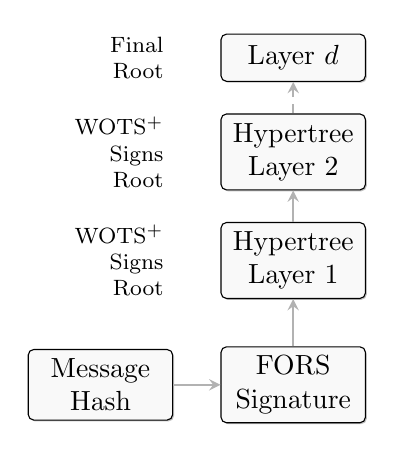
\begin{tikzpicture}[
      block/.style={
        rectangle,
        draw,
        fill=white,
        text width=1.6cm,
        align=center,
        minimum height=0.6cm,
        rounded corners=2pt,
        fill=gray!5,
        drop shadow={shadow xshift=0.5pt, shadow yshift=-0.5pt}
      },
      arrow/.style={->,>=stealth,thick,draw=gray!60},
      level/.style={sibling distance=35mm,level distance=0.7cm}
    ]
    % Message and Components
    \node[block] (fors) at (0,0) {FORS\\Signature};
    \node[block,left=0.6cm of fors] (hash) {Message\\Hash};

    % Hypertree Layers
    \node[block,above=0.6cm of fors] (ht1) {Hypertree\\Layer 1};
    \node[block,above=0.4cm of ht1] (ht2) {Hypertree\\Layer 2};
    \node[block,above=0.4cm of ht2] (htd) {Layer $d$};

    \draw[arrow] (hash) to (fors);
    \draw[arrow] (fors) to (ht1);
    \draw[arrow] (ht1) to (ht2);
    \draw[arrow] ($(htd)+(0,-0.5)$) -- (htd);
    \draw[dashed,thick,gray!60] ($(ht2)+(0,0.5)$) -- ($(htd)+(0,-0.3)$);

    \node[left=0.6cm of ht1,text width=1.4cm,font=\footnotesize,align=right] {WOTS\textsuperscript{+} Signs Root};
    \node[left=0.6cm of ht2,text width=1.4cm,font=\footnotesize,align=right] {WOTS\textsuperscript{+} Signs Root};
    \node[left=0.6cm of htd,text width=1.4cm,font=\footnotesize,align=right] {Final Root};
  \end{tikzpicture}
  \caption{SLH-DSA signature generation flow.}
  \label{fig:sphincs-process}
\end{figure}

The SLH-DSA signature generation process, illustrated in Fig.~\ref{fig:sphincs-process}, implements a hierarchical authentication structure. Initially, a message digest is generated through hashing, followed by FORS few-time scheme signing, which produces $k$ authentication paths comprising $t$ elements each. The resulting FORS public key undergoes authentication via a $d$-layer hypertree, where each layer applies WOTS\textsuperscript{+} to sign the lower layer's root. This signature chain terminates at the final root node, enabling efficient verification while maintaining robust hash-based security.

\textcolor{blue}{SLH-DSA offers ``small'' (s) and ``fast'' (f) operational modes, where ``small'' denotes reduced signature size and ``fast'' indicates higher signature generation speed, across different parameter sets and security levels \cite{Barker}. }
Various parameter sets accommodate different requirements regarding signature size, security level, and computational efficiency. All security properties are derived from underlying hash functions, providing resistance to quantum computational attacks.

\subsection{GPU Computing Model}

Graphics Processing Units (GPUs) incorporate numerous cores organized within Streaming Multiprocessors (SMs). This parallel architecture implements Single Instruction, Multiple Thread (SIMT) execution, organizing threads into warps that collectively form blocks. These blocks are distributed across available SMs, enabling thousands of concurrent threads to execute similar instructions simultaneously.

The CUDA framework enhances computational throughput through memory optimization strategies including coalesced memory accesses, shared memory utilization, and constant memory buffering. These techniques facilitate extensive parallelization of SLH-DSA computations, yielding performance improvements through the combined application of thread-level, data-level, and algorithmic parallelism.

\section{Optimized Implementation of SLH-DSA}\label{sec:implementation}

The thread-adaptive parallelization architecture for SLH-DSA, illustrated in Fig.~\ref{fig:optimization_architecture}, consists of three hierarchical layers. The top layer represents cryptographic operations, with the Sign operation emphasized. The middle layer applies Adaptive Thread Allocation (ATA), distributing dynamically optimized thread configurations across $t$ parallel instances. The bottom layer employs Function-Level Parallelism (FLP), decomposing operations into algorithmic components—FORS, WOTS\textsuperscript{+}, and Hypertree—with each component mapped to multiple GPU warps of 32 threads. This structure enables efficient resource utilization and fine-grained parallel execution for SLH-DSA on GPU platforms.

\begin{figure}[htbp]
  \centering
  \resizebox{0.48\textwidth}{!}{
    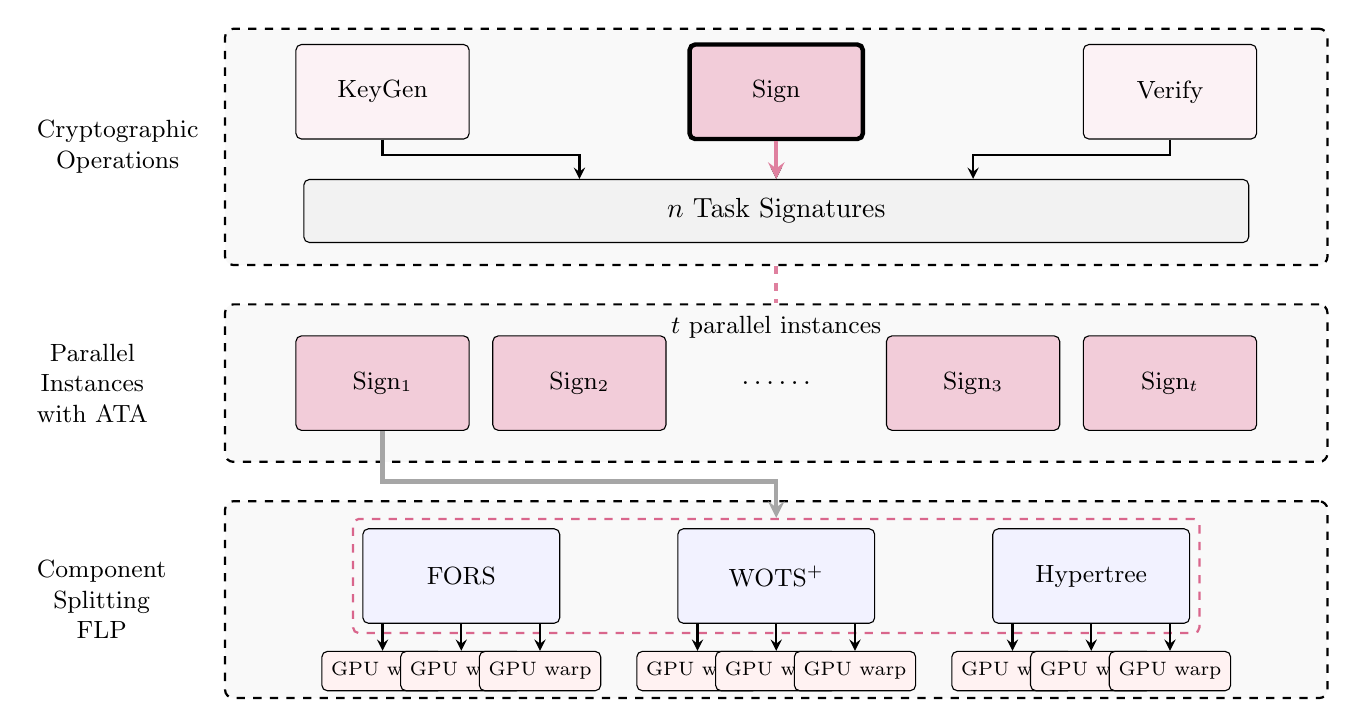
\begin{tikzpicture}[
        % Define styles with better semantic meaning
        layer/.style={draw, rounded corners=3pt, dashed, thick, fill=gray!5, minimum width=14cm, minimum height=2.5cm},
        task/.style={draw, rounded corners=2pt, minimum width=2.2cm, minimum height=1.2cm, align=center, font=\small, fill=purple!5},
        selected/.style={task, fill=purple!20, ultra thick},
        component/.style={draw, rounded corners=2pt, minimum width=2.5cm, minimum height=1.2cm, align=center, font=\small, fill=blue!5},
        gpu/.style={draw, rounded corners=2pt, minimum width=1.1cm, minimum height=0.5cm, font=\scriptsize, align=center, fill=red!5},
        arrow/.style={->, >=stealth, thick},
        manyarrows/.style={->, >=stealth, thick, draw=gray!70},
        highlightarrow/.style={->, >=stealth, thick, draw=purple!60, dashed},
        highlightbox/.style={draw, rounded corners=2pt, dashed, thick, draw=purple!60, fit=#1}
      ]

      % Layer boxes with vertical stacking
      \node[layer, anchor=north, minimum width=14cm, minimum height=3cm] (layer1) at (0,4.5) {};
      \node[layer, anchor=north, minimum width=14cm, minimum height=2cm] (layer2) at (0,1.0) {};
      \node[layer, anchor=north] (layer3) at (0,-1.5) {};

      % Layer labels - positioned relative to each layer
      \node[align=center, font=\small, anchor=west] at ($(layer1.west) + (-2.5,0)$) {Cryptographic\\Operations};
      \node[align=center, font=\small, anchor=west] at ($(layer2.west) + (-2.5,0)$) {Parallel\\Instances\\with ATA};
      \node[align=center, font=\small, anchor=west] at ($(layer3.west) + (-2.5,0)$) {Component\\Splitting\\FLP};

      % Signature tasks with horizontal positioning in top layer
      \node[task] (keygen) at ($(layer1.center) + (-5,0.7)$) {KeyGen};
      \node[selected] (sign) at ($(layer1.center) + (0,0.7)$) {Sign};
      \node[task] (verify) at ($(layer1.center) + (5,0.7)$) {Verify};

      % Task queue - positioned relative to the layer
      \node[draw, rounded corners=2pt, fill=gray!10, minimum width=12cm, minimum height=0.8cm]
      (queue) at ($(layer1.south) + (0,0.7)$) {$n$ Task Signatures};

      % Connect tasks to queue using relative positioning
      \foreach \op/\pos in {keygen/-5, sign/0, verify/5} {
        \draw[arrow] (\op) -- ++(0,-0.8) -| ($(queue.north) + (\pos/2,0)$);
      }

      % Highlight the selected task path
      \draw[arrow, ultra thick, draw=purple!50] (sign) -- ++(0,-0.8) -| (queue);

      % Changed to dashed line for middle arrow
      \draw[ultra thick, draw=purple!50, dashed] (layer1.south) -- ($(layer2.north) + (0,0)$);

      % Label for instances - positioned relative to the connection
      \node[font=\small] at ($(layer2.north) + (0,-0.3)$) {$t$ parallel instances};

      % Multiple instances of sign task - positioned relative to middle layer
      \foreach \i/\pos in {1/-5,2/-2.5,3/2.5} {
        \node[task, fill=purple!20] (sign\i) at ($(layer2.center) + (\pos,0)$) {Sign$_{\i}$};
      }
      \node[task, fill=purple!20] (signt) at ($(layer2.center) + (5,0)$) {Sign$_{t}$};

      \node at ($(layer2.center) + (0,0)$) {$\ldots \ldots$};

      % Component splitting - positioned relative to bottom layer
      \node[component] (fors) at ($(layer3.center) + (-4,0.3)$) {FORS};
      \node[component] (wots) at ($(layer3.center) + (0,0.3)$) {WOTS\textsuperscript{+}};
      \node[component] (hypertree) at ($(layer3.center) + (4,0.3)$) {Hypertree};

      % Highlight Sign1 expanding to FLP layer
      \node[highlightbox={(fors) (wots) (hypertree)}] (flpbox) {};
      \draw[manyarrows, ultra thick] (sign1.south) -- ($(layer2.south)!0.5!(layer3.north) + (-5,0)$) --
      ($(layer2.south)!0.5!(layer3.north) + (0,0)$) -- (flpbox.north);

      % GPU Blocks - positioned relative to components
      \foreach \comp/\name/\pos in {fors/FORS/-4, wots/WOTS/0, hypertree/Hypertree/4} {
        \foreach \shift in {-1, 0, 1} {
          \node[gpu] (gpu\name\shift) at ($(\comp.south) + (\shift,-0.6)$) {GPU warp};
          \draw[arrow] ($(\comp.south) + (\shift,-0.0)$) -- (gpu\name\shift);
        }
      }

    \end{tikzpicture}
  }
  \caption{Thread-adaptive parallelization architecture for SLH-DSA.}
  \label{fig:optimization_architecture}
\end{figure}

\subsection{Adaptive Thread Allocation}

Thread-Adaptive allocation methodology through precise calibration of thread counts based on empirical performance models, establishing function-specific optimal configurations that balance parallelizable workload against synchronization costs. Performance gains are achieved through the elimination of thread contention in complex operations and reduction of management overhead in simpler functions, resulting in improved overall system throughput.

\subsubsection{Performance Modeling}

The execution time for each cryptographic function $g_i$ in SLH-DSA is characterized by:

\begin{equation}
  \label{eq:execution_time_model}
  T(g_i, t) = \alpha_i + \frac{\beta_i}{t} + \gamma_i \cdot t,
\end{equation}
This model captures three essential components: $\alpha_i$ represents invariant computational overhead independent of thread count, $\frac{\beta_i}{t}$ reflects the parallelizable workload component that scales inversely with thread count, and $\gamma_i \cdot t$ quantifies thread management overhead that increases linearly with thread allocation. The formulation encapsulates the fundamental parallelization tradeoff between computational acceleration and synchronization costs.

\subsubsection{Optimal Thread Determination}

By minimizing $T(g_i, t)$ with respect to $t$, the optimal thread allocation $t_i^*$ for each function is derived as:

\begin{equation}
  \label{eq:optimal_thread_count}
  t_i^* = \sqrt{\frac{\beta_i}{\gamma_i}},
\end{equation}
The parameters $\alpha_i$, $\beta_i$, and $\gamma_i$ were determined through systematic profiling of each cryptographic operation across multiple thread configurations, establishing an empirical foundation for optimization decisions.

\subsubsection{Thread Configuration Optimization}

\color{blue}
The thread allocation optimization methodology is presented in Algorithm~\ref{alg:adaptive_thread_allocation}, which profiles each cryptographic function across thread configurations from $2^{11}$ to $2^{17}$. Performance data is fitted to the analytical model in Equation~(\ref{eq:execution_time_model}), determining parameters $\alpha_i$, $\beta_i$, and $\gamma_i$. The theoretically optimal thread count is calculated and rounded to the nearest power of two for GPU warp alignment. This approach optimizes resource allocation for each cryptographic operation, minimizing execution time across the signature generation workflow.
\color{black}

\begin{algorithm}
  \caption{Thread Configuration Optimization}
  \label{alg:adaptive_thread_allocation}
  \color{blue}
  \begin{algorithmic}[1]
    \REQUIRE Set of cryptographic functions $G = \{g_1, g_2, \ldots, g_m\}$
    \ENSURE Optimized thread configuration for each function

    \STATE Initialize $\textsf{ThreadConfig}[\,] \gets \emptyset$
    \FOR{$g_i \in G$}
    \STATE $\textsf{ThreadCounts} \gets \{2^{11}, 2^{12}, 2^{13}, 2^{14}, 2^{15}, 2^{16}, 2^{17}\}$
    \STATE $\textsf{PerfData} \gets \textsf{PROFILE}(g_i, \textsf{ThreadCounts})$
    \STATE $(\alpha_i, \beta_i, \gamma_i) \gets \textsf{FIT\_MODEL}(\textsf{PerfData})$
    \STATE $t_{\textsf{opt}} \gets \sqrt{\frac{\beta_i}{\gamma_i}}$
    \STATE $t_i^* \gets \textsf{ROUND\_POWER2}(t_{\textsf{opt}})$
    \STATE $\textsf{ThreadConfig}[g_i] \gets t_i^*$
    \ENDFOR

    \RETURN $\textsf{ThreadConfig}$
  \end{algorithmic}
\end{algorithm}

\subsection{Function-Level Parallelism}

\color{blue}

Function-Level Parallelism  decomposes cryptographic operations into granular computational tasks that can be executed concurrently rather than treating them as atomic units. This approach enables fine-grained parallelization across multiple execution threads, resulting in reduced cryptographic latency through optimal resource utilization. The implementation applies this methodology to the three core components of SLH-DSA: WOTS$^+$, FORS, and Hypertree.

\subsubsection{WOTS\texorpdfstring{$^+$}{+} Parallelization}

The WOTS$^+$ implementation facilitates concurrent computation of $l$ independent hash chains by allocating individual chains or chain segments to distinct GPU threads. After hash chain computation completion, results are consolidated into leaf nodes using GPU shared memory rather than global memory to minimize access latencies. For hypertree structures, multiple Merkle tree WOTS$^+$ public keys are generated simultaneously, with shared memory buffers optimizing authentication path construction. This approach differs significantly from previous implementations \cite{Kim2024}.

\subsubsection{FORS Parallelization}

The FORS component implementation employs fine-grained parallelism for generating $k \times 2^a$ secret key elements and leaf nodes concurrently. Multiple Merkle trees are constructed simultaneously, with each of the $k$ trees assigned to independent thread blocks. Shared memory buffers are strategically employed during tree construction to aggregate intermediate roots, significantly reducing global memory access operations during public key derivation. This approach builds upon methodologies established in \cite{Wang2025} while enhancing memory utilization patterns for the specific characteristics of the FORS structure.

\subsubsection{Hypertree Parallelization}

For the hypertree construction, parallel processing is applied across multiple Merkle trees spanning all $d$ layers. The leaf nodes are initially generated through parallel hash chain computations before being consolidated into tree structures. Due to shared memory constraints preventing full parallelization of all nodes across all layers, a semi-parallel approach was implemented. This methodology differs from the full-node parallelization presented in \cite{Wang2025} by employing a hierarchical execution strategy where each thread processes four-node combinations rather than two-node combinations, thereby reducing synchronization overhead.

\color{black}

\section{Performance Evaluation}\label{sec:evaluation}

\subsection{Experimental Setup}

Evaluation was conducted on standardized hardware platforms to facilitate comparative analysis. The experimental configuration comprised the following components: an NVIDIA RTX 4090 GPU with 24GB GDDR6X memory, operating under Ubuntu 24.04 LTS. Compilation was performed using CUDA 12.5 and GCC 13.3.0.
Testing utilized standardized NIST parameter sets for SLH-DSA at security levels 1 and 3, corresponding to 128 and 192 bits of security. Each measurement was replicated 20 times, with statistical outliers removed using median absolute deviation techniques.

\subsection{Comparative Performance Analysis}

The implementation was benchmarked against state-of-the-art alternatives using SHA2-128f parameters. Table \ref{tab:comparative_perf} presents latency and throughput metrics across comparable hardware platforms.
Consistent performance improvements were observed across all cryptographic operations compared to reference implementations on identical hardware. 
\textcolor{blue}{For SHA2-128f, key generation, signature generation, and verification latencies were reduced, and corresponding throughput was increased. Specifically, compared to Kim et al.~\cite{Kim2024}, the throughput of our implementation is 2.20$\times$ for key generation, 1.41$\times$ for signature generation, and 1.76$\times$ for verification. Compared to Wang et al.~\cite{Wang2025}, the throughput is 1.11$\times$, 1.16$\times$, and 1.43$\times$ for key generation, signature generation, and verification, respectively, on the same hardware (RTX 4090).}

\begin{table*}[htpb]
  \centering
  \caption{Performance Comparison of SLH-DSA Implementations}
  \label{tab:comparative_perf}
  \begin{tabular}{@{}lccccccc@{}}
    \toprule
    \multirow{2}{*}{\textbf{Parameter Sets, Year [Work], Tasks}} & \multicolumn{3}{c}{\textbf{Latency (ms)}} & \multicolumn{3}{c}{\textbf{Throughput (tasks/sec)}} & \multirow{2}{*}{\textbf{Device}} \\
    \cmidrule(lr){2-4} \cmidrule(lr){5-7}
    & \textbf{KG} & \textbf{Sign} & \textbf{Verify} & \textbf{KG} & \textbf{Sign} & \textbf{Verify} & \\
    \midrule
    SHA2-128f, 2024 \cite{Kim2024}, 512  & 0.71 & 11.53 & 1.79 & 725,118 (55\%) & 44,391 (97\%) & 285,681 (81\%) & RTX 3090 \\
    SHA2-128f, 2025 \cite{Wang2025}, 41,984 & 32.07 & 924.24 & 119.16 & 1,309,136 (100\%) & 45,425 (100\%) & 352,333 (100\%) & RTX 3090 \\
    SHA2-128f, 2025 \cite{Wang2025}$^\dagger$, 32,768 & 22.82 & 609.03 & 72.51 & 1,435,690 (109.7\%) & 53,804 (118.4\%) & 451,883 (128.3\%) & RTX 4090 \\
    SHA2-128f, This work, 32,768 & 20.64 & 526.48 & 65.24 & \textbf{1,587,849} (\textbf{121.3\%}) & \textbf{62,239} (\textbf{137.0\%}) & \textbf{502,243} (\textbf{142.5\%}) & RTX 4090 \\
    \bottomrule
  \end{tabular}
  \begin{tablenotes}
  \item[] $\dagger$: Results obtained by executing previously published implementations on the RTX 4090 test environment for direct hardware-equivalent comparison.
  \end{tablenotes}
\end{table*}

\subsection{Thread Allocation Efficiency}

ATA efficacy was evaluated through execution time measurements across varying thread configurations for core cryptographic functions. Table \ref{tab:thread_model_params} presents experimentally derived model parameters and optimal thread allocations.

\begin{table}[h]
  \centering
  \caption{Thread Model Parameters and Optimal Allocations}
  \label{tab:thread_model_params}
  \begin{tabular}{@{}lrrrr@{}}
    \toprule
    \textbf{Operation} & \boldmath$\alpha_i$ & \boldmath$\beta_i$ & \boldmath$\gamma_i$ & \boldmath$t_i^*$ \\
    \midrule
    SHA2-128f-keygen & 52.06 & 506,000.57 & 1.26E-4 & 63,310 \\
    SHA2-128f-sign & 1386.01 & 13,231,567.75 & 3.60E-3 & 60,636 \\
    SHA2-128f-verify & 164.72 & 1,395,012.54 & 4.54E-4 & 55,407 \\
    SHA2-128s-keygen & 3317.74 & 32,046,199.26 & 7.15E-3 & 66,929 \\
    SHA2-128s-sign & 23716.81 & 248,632,501.64 & 6.59E-2 & 61,419 \\
    SHA2-128s-verify & 63.22 & 484,914.46 & 1.44E-4 & 57,968 \\
    SHA2-192f-keygen & 79.37 & 822,859.78 & 2.40E-4 & 58,560 \\
    SHA2-192f-sign & 2319.70 & 23,961,551.63 & 8.55E-3 & 52,932 \\
    SHA2-192f-verify & 267.63 & 2,342,878.75 & 8.91E-4 & 51,274 \\
    \bottomrule
  \end{tabular}
\end{table}

\color{blue}

The execution time model parameters reveal distinct characteristics across cryptographic operations. The $\alpha_i$ parameter quantifies non-parallelizable sequential overhead, with sign operations exhibiting substantially higher values (e.g., SHA2-128s-sign: 23716.81) than key generation and verification operations. The $\beta_i$ coefficient represents parallelizable workload components, with higher values indicating greater potential performance gain from increased parallelism. The $\gamma_i$ parameter measures synchronization and thread management overhead, which increases with thread count.

According to equation (\ref{eq:optimal_thread_count}), operations with higher $\beta_i/\gamma_i$ ratios yield higher optimal thread counts. Experimental validation confirms performance degradation of 18-23\% when exceeding optimal thread allocation ($t_i^*$) and significant latency increases when using insufficient threads. Notable consistency in optimal thread allocation is observed within parameter sets (e.g., 55,407-63,310 for SHA2-128f), while security level transitions show distinct allocation patterns, reflecting fundamental algorithmic characteristics.

\color{black}

\subsection{Function-Level Parallelism Impact}

\begin{figure}[h]
  \centering
  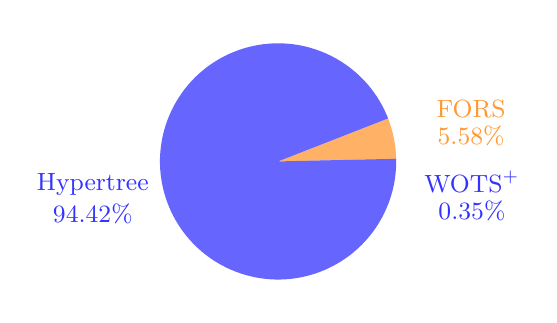
\begin{tikzpicture}
    % Pie chart: values are percentages
    \def\wots{0.35}
    \def\fors{5.58}
    \def\hypertree{94.42}
    \def\startAngle{0}
    % WOTS+ slice
    \fill[blue!40] (0,0) -- (\startAngle:1.5) arc (\startAngle:\startAngle+\wots*3.6:1.5) -- (0,0);
    \pgfmathsetmacro\angleA{\startAngle+\wots*3.6}
    % FORS slice
    \fill[orange!60] (0,0) -- (\angleA:1.5) arc (\angleA:\angleA+\fors*3.6:1.5) -- (0,0);
    \pgfmathsetmacro\angleB{\angleA+\fors*3.6}
    % Hypertree slice
    \fill[blue!60] (0,0) -- (\angleB:1.5) arc (\angleB:\angleB+\hypertree*3.6:1.5) -- (0,0);

    % Labels
    \node[blue!80, font=\small] at ({\startAngle-0.5*\fors*3.6}:2.5) {\shortstack{WOTS\textsuperscript{+}\\ 0.35\%}};
    \node[orange!80, font=\small] at ({\angleA+0.5*\fors*3.6}:2.5) {\shortstack{FORS\\5.58\%}};
    \pgfmathsetmacro{\hypertreeAngle}{\angleB+0.5*\hypertree*3.6}
    \node[blue!80, font=\small] at (\hypertreeAngle:2.4) {\shortstack{Hypertree \\ 94.42\%}};
  \end{tikzpicture}
  \caption{Signing latency breakdown for SHA2-128f.}
  \label{fig:flp_pie}
\end{figure}

Analysis indicates that Hypertree construction dominates signing latency, accounting for 94.42\% of total execution time (497.11 ms), while FORS and WOTS\textsuperscript{+} contribute 5.58\% (29.37 ms) and 0.35\% (1.857 ms), respectively, as visually depicted in Fig.~\ref{fig:flp_pie}. Despite FLP optimizations of individual hash computations, inherent sequential dependencies and operation volume in the Hypertree constrain achievable parallelism compared to FORS and WOTS\textsuperscript{+} components. This observation highlights the necessity for targeted optimization of Hypertree structures for future performance enhancements.

\subsection{Scalability Analysis}

Implementation scalability was evaluated across varying security parameters and computational complexities. Table \ref{tab:scalability} presents execution metrics for signature generation across different parameter sets.

\begin{table}[h]
  \centering
  \caption{Scalability Across SLH-DSA Signature Parameter Sets}
  \label{tab:scalability}
  \begin{tabular}{@{}lcc@{}}
    \toprule
    \textbf{Parameter Set} & \textbf{Latency (ms)} & \textbf{Throughput (tasks/sec)} \\
    \midrule
    SHA2-128s \cite{Wang2025} & 12,185.35 & 2,689 \\
    SHA2-128s & 9,125.94 & 3,591 \\
    \midrule
    SHA2-192f \cite{Wang2025} & 1,067.26 & 30,703 \\
    SHA2-192f & 977.45 & 33,524 \\
    \midrule
    SHA2-192s \cite{Wang2025} & 21,252.11 & 1,542 \\
    SHA2-192s & 18,711.43 & 1,751 \\
    \bottomrule
  \end{tabular}
\end{table}

Superior performance was observed across all parameter configurations, with notable improvements for robust variants. The SHA2-128s parameter set exhibited a 25\% latency reduction and 33.5\% throughput enhancement. Thread-adaptive techniques proved most effective for computationally intensive operations with smaller hash sizes. Diminishing returns were observed at higher security levels due to increased synchronization overhead, reflecting an inherent trade-off between security parameters and parallel execution efficiency.

\section{Conclusion}\label{sec:conclusion}

A thread-adaptive GPU implementation of SLH-DSA was developed that dynamically allocates computational resources based on cryptographic function profiles while decomposing operations into finely-grained parallel tasks. Performance evaluation on an NVIDIA RTX 4090 GPU demonstrated a throughput of 62,239 signatures per second for SHA2-128f parameters, representing a 15.68\% improvement over state-of-the-art implementations. Empirical analysis identified Hypertree construction as the primary performance bottleneck, accounting for 94\% of signing latency despite component-level optimizations. The implementation exhibited particular efficacy for robust parameter variants, with SHA2-128s showing a 25\% latency reduction and 33.5\% throughput enhancement. These results establish GPU platforms as viable acceleration frameworks for post-quantum cryptographic schemes. Future work will focus on Hypertree structure optimization and performance evaluation across diverse GPU architectures.

% \section*{Acknowledgments}

% {\appendix[Proof of the Zonklar Equations]
% Use $\backslash${\tt{appendix}} if you have a single appendix:
% Do not use $\backslash${\tt{section}} anymore after $\backslash${\tt{appendix}}, only $\backslash${\tt{section*}}.
% If you have multiple appendixes use $\backslash${\tt{appendices}} then use $\backslash${\tt{section}} to start each appendix.
% You must declare a $\backslash${\tt{section}} before using any $\backslash${\tt{subsection}} or using $\backslash${\tt{label}} ($\backslash${\tt{appendices}} by itself
%  starts a section numbered zero.)}

%{\appendices
%\section*{Proof of the First  Equation}
%Appendix one text goes here.
% You can choose not to have a title for an appendix if you want by leaving the argument blank
%\section*{Proof of the Second  Equation}
%Appendix two text goes here.}

% argument is your BibTeX string definitions and bibliography database(s)
\bibliography{biblio}

\bibliographystyle{IEEEtran}

% \newpage

% % \bf{If you include a photo:}\vspace{-33pt}
% \begin{IEEEbiography}[{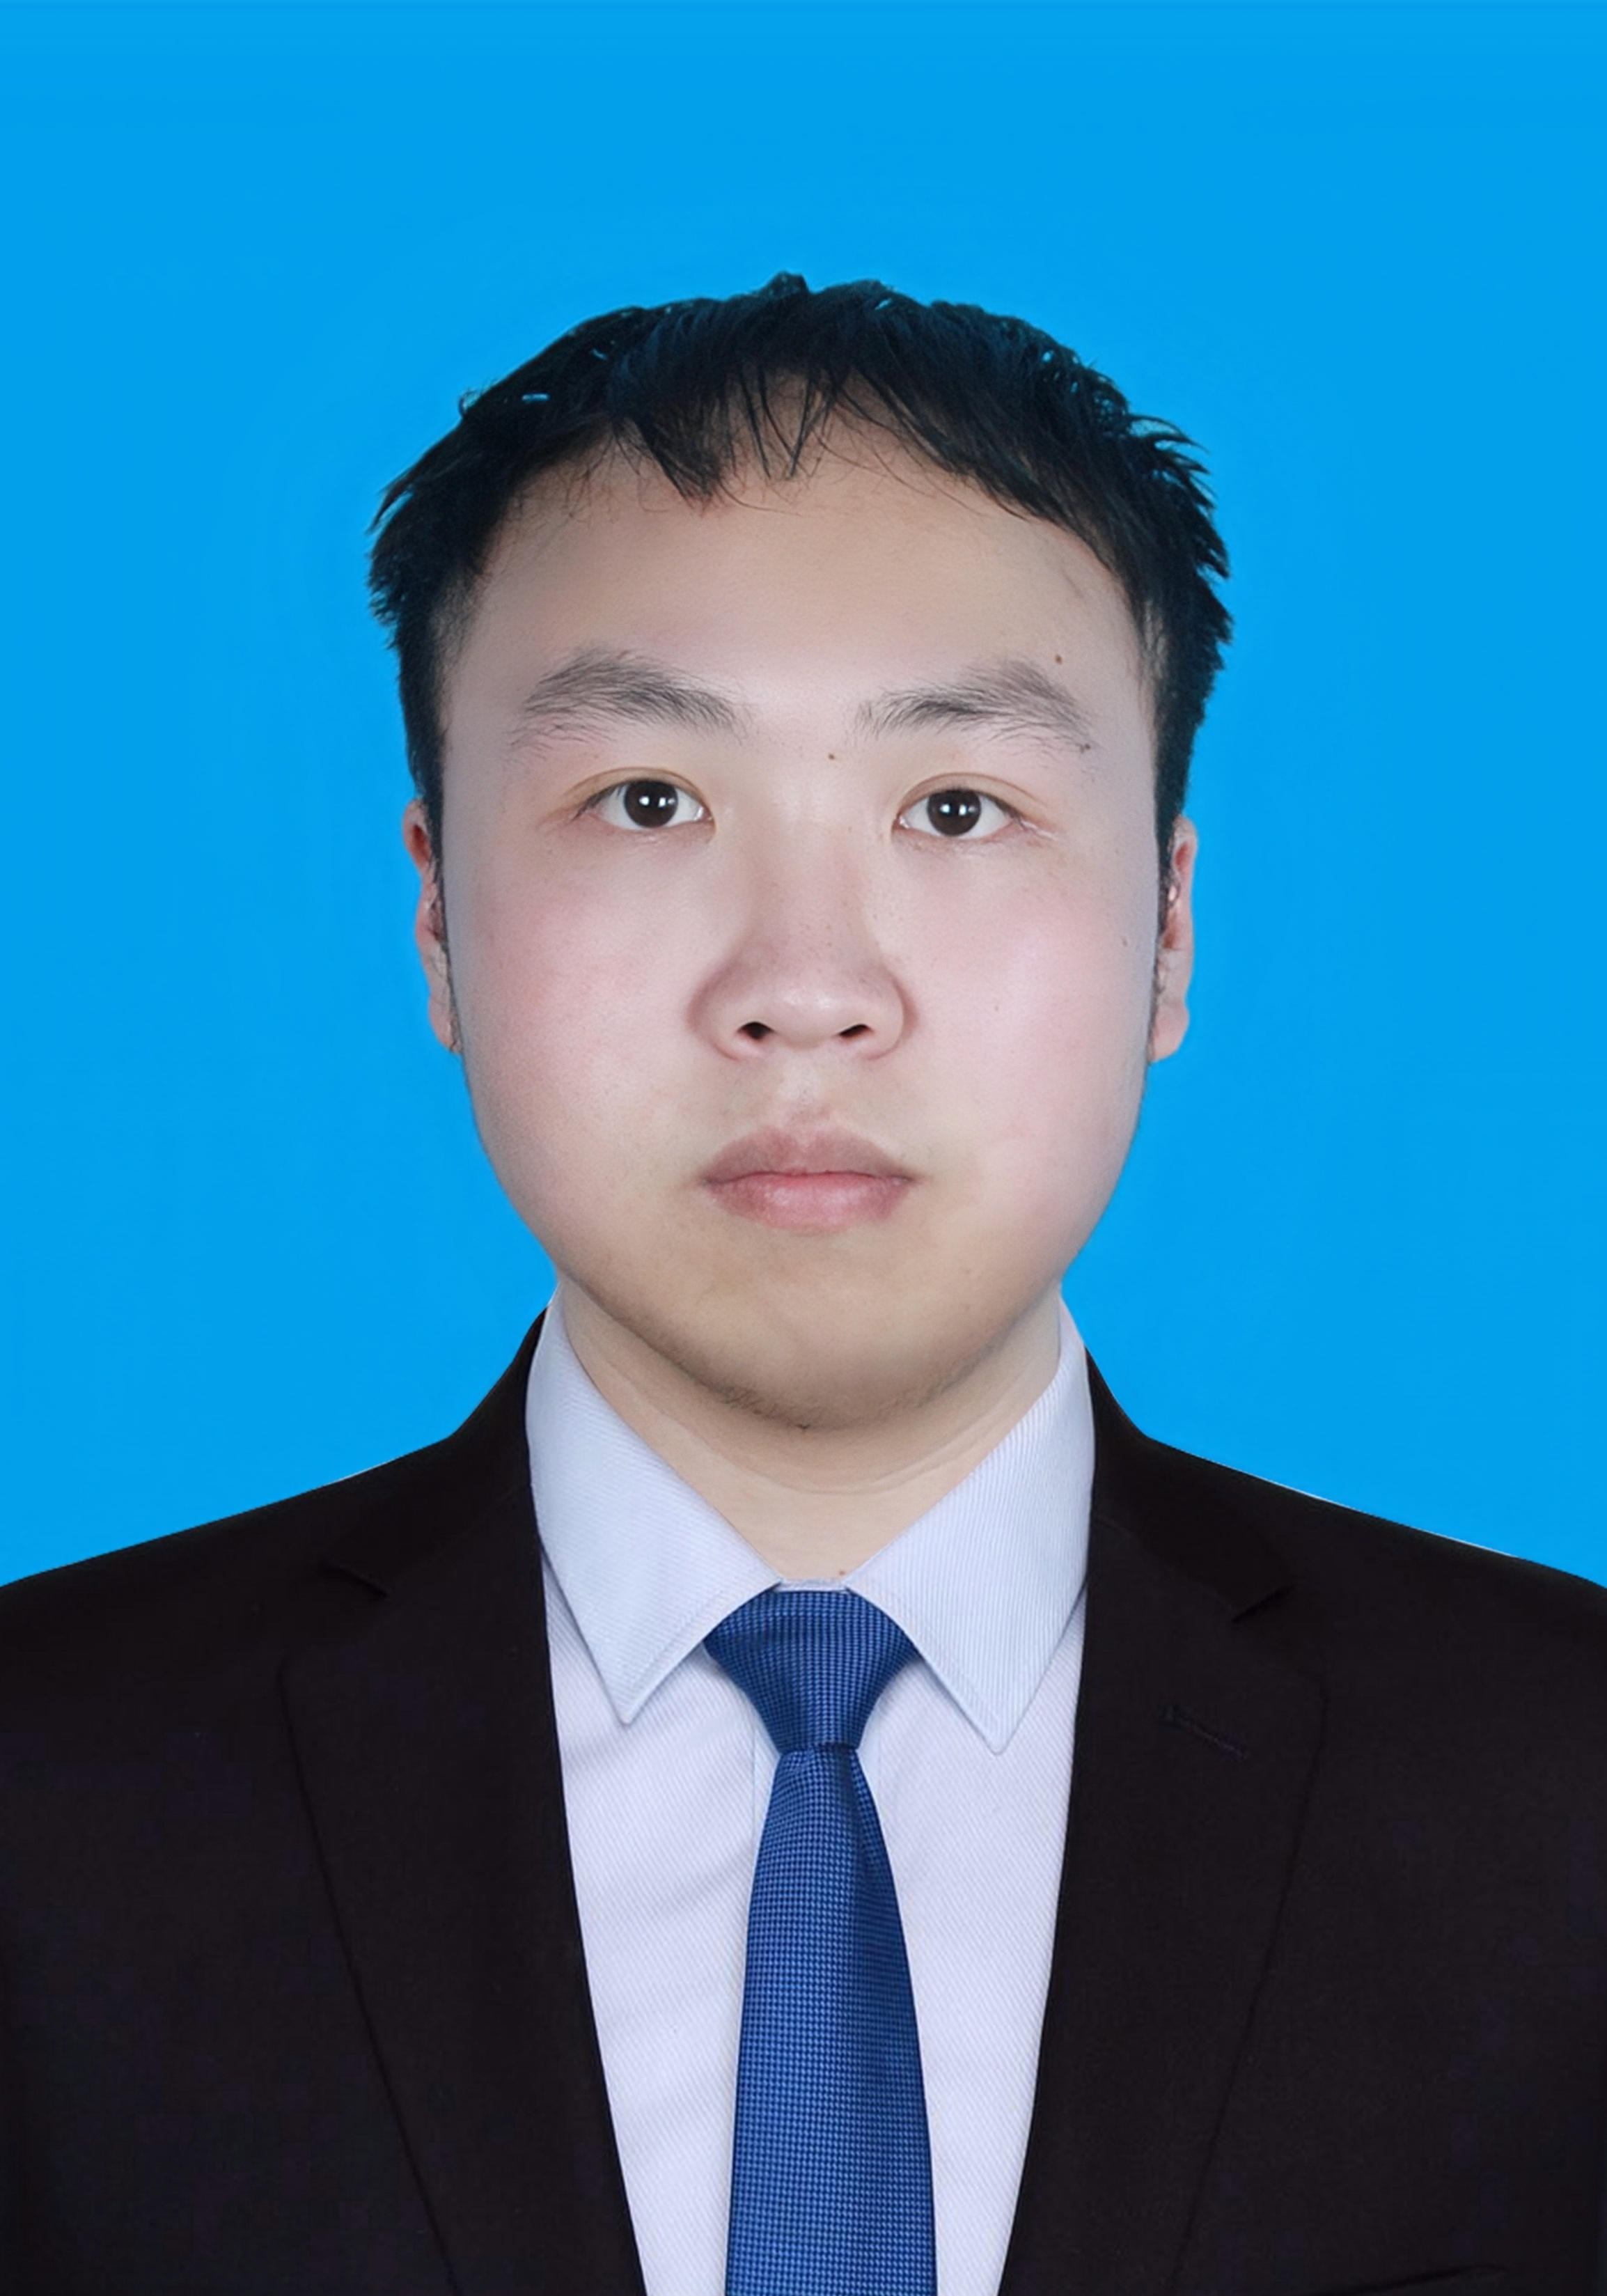
\includegraphics[width=1in,height=1.25in,clip,keepaspectratio]{./fig/self.jpg}}]{Jiahao Xiang}
%   is pursuing a Master's degree in Electronic Information at Hengyang Normal University, China. His research focuses on cryptographic engineering and efficient implementations of block ciphers on resource-constrained devices. Publications include works on lightweight cryptography optimization and contributions to open-source cryptographic projects.
% \end{IEEEbiography}

% \begin{IEEEbiography}[{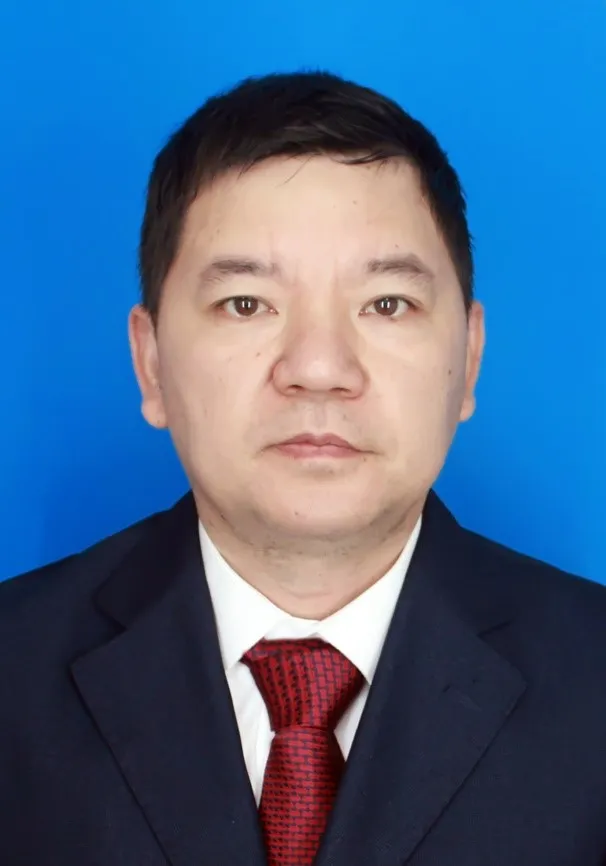
\includegraphics[width=1in,height=1.25in,clip,keepaspectratio]{./fig/boss.png}}]{Lang Li}
%   received his Ph.D. and Master's degrees in computer science from Hunan University, Changsha, China, in 2010 and 2006, respectively, and earned his B.S. degree in circuits and systems from Hunan Normal University in 1996. Since 2011, he has been working as a professor in the College of Computer Science and Technology at the Hengyang Normal University, Hengyang, China. He has research interests in embedded system and information security.
% \end{IEEEbiography}

% \vspace{11pt}

% \bf{If you will not include a photo:}\vspace{-33pt}
% \begin{IEEEbiographynophoto}{Jiahao Xiang}
%   is pursuing a Master's degree in Electronic Information at Hengyang Normal University, China. His research focuses on cryptographic engineering and efficient implementations of block ciphers on resource-constrained devices. Publications include works on lightweight cryptography optimization and contributions to open-source cryptographic projects.
% \end{IEEEbiographynophoto}

% \begin{IEEEbiographynophoto}{Lang Li}
%   received his Ph.D. and Master's degrees in computer science from Hunan University, Changsha, China, in 2010 and 2006, respectively, and earned his B.S. degree in circuits and systems from Hunan Normal University in 1996. Since 2011, he has been working as a professor in the College of Computer Science and Technology at the Hengyang Normal University, Hengyang, China. He has research interests in embedded system and information security.
% \end{IEEEbiographynophoto}

\end{document}